\section{Thursday, June 13}

\todaybox{ We will continue our discussion of primitives, to prove that analytic functions have primitives under certain conditions.

We will also lay out a general framework for integration, detailing where we're going in the following weeks.}

The conditions on the curves in our CIT version 2 and in theorem \ref{thm:pathind} -- namely that the domain contains all regions bounded by the curve -- are generally annoying to handle on a case by case basis. And if we want our strategy to find a primitive to work, we need these conditions to hold for all curves from $z_0$ to $z$ in $D$. So we should expect this to require a condition on $D$. Fortunately, there's a nice topological condition we can impose that guarantees everything we need.

\begin{defbo}{Simply Connected Domains}{}\index{Domain!simply connected}

A domain $D$ is called simply connected if for every simple, closed curve $\gamma$ in $D$, that $\mathrm{in}(\gamma) \subset D$.

\end{defbo}

Intuitively, this means that the set has no "holes". For example:

\begin{ex}{}{} These domains are not simply connected because they have "holes":

\begin{center}
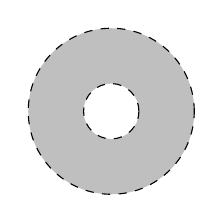
\begin{tikzpicture}[baseline=(current bounding box.center)]

\draw[fill = lightgray, dashed] (0,0) circle (30pt);
\draw[dashed, fill = white] (0,0) circle (10pt);

\end{tikzpicture}
\qquad or \qquad
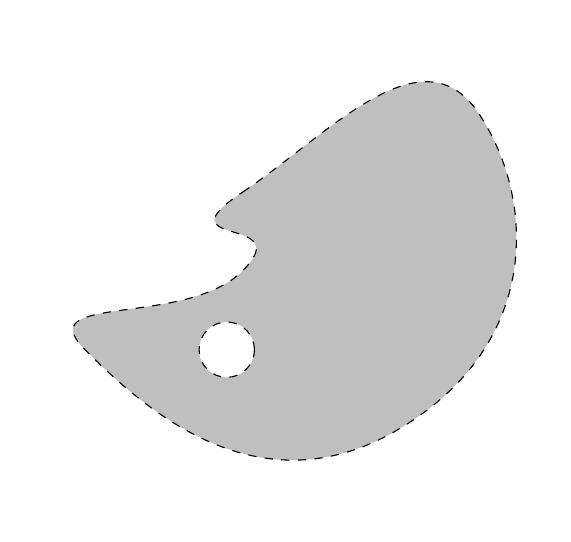
\begin{tikzpicture}[baseline=(current bounding box.center)]


\draw[dashed, fill = lightgray] plot [smooth cycle, tension = 1.3] coordinates {(0,0)  (0,1) (3,2) (2,-2) (-2,-1)};
\draw[dashed, fill = white] (-0.2,-1) circle (10pt);
\end{tikzpicture}

\end{center}

On the other hand, there are plenty of sets we're used to that are simply connected. $\C$, $\C\setminus (-\infty,0]$, and any open ball are all simply connected.
\end{ex}

This condition lets us state another version of the Cauchy Integral Theorem:

\begin{thmbo}{Cauchy's Integral Theorem (version 3)}{cit3}\index{Cauchy's Integral Theorem!version 3} Suppose $f(z)$ is analytic on a simply connected domain $D$. If $\gamma$ is any piecewise smooth, closed curve in $D$, then:

$$\int_{\gamma}f(z)dz = 0$$
\end{thmbo}

\begin{proof} This follows immediately from CIT version 2, since any closed curve in a simply connected domain satisfies the hypotheses of CIT version 2.\end{proof}

Having a sufficiently general version of the Cauchy Integral Theorem is a key step towards proving results about primitives. However, before we do that, we need another result. As it turns out, the result guaranteeing primitives that I would like to prove hinges on the ability to estimate integrals. So, before we can finish talking about primitives, we need the following result:

\begin{thmbo}{M-L Estimation of Integrals}{mlest}\index{M-L estimate} Suppose $\gamma:[a,b]\rightarrow \C$ is a piecewise smooth curve and $f(z)$ is a continuous function whose domain includes $\gamma$. Let $M = \max\left\{|f(\gamma(t))|\middle|t\in[a,b]\right\}$, and $L = \mathrm{Length}(\gamma)$. Then:
$$\left|\int_{\gamma}f(z)dz\right| \le ML$$
\end{thmbo}

\begin{proof} To begin, we will need to prove a nice fact: for any curve $g:[a,b]\rightarrow \C$, we have:
$$\left|\int_a^b g(t)dt\right| \le \int_a^b|g(t)|dt$$

Let $\int_a^bg(t)dt = re^{i\theta}$. Set $h(t) = e^{-i\theta}g(t)$. Then:
$$\int_a^bh(t)dt = \int_a^b e^{-i\theta}g(t)dt = e^{-i\theta}\int_a^bg(t)dt = r$$

So $\int_a^bh(t)dt \in \R$. We therefore have that $\RE\int_a^bh(t)dt = \int_a^b\RE(h(t))dt$. So, we have:

\begin{align*}\left|\int_a^bg(t)dt\right| &= r\\
&= \left|\int_a^b h(t)dt\right|\\
&= \left|\int_a^b \RE(h(t))dt\right|\\
&\le \int_a^b \left|\RE(h(t))\right|dt \hspace{30pt} (\text{from multivariable calc})\\
&\le \int_a^b |h(t)|dt \hspace{55pt} (\text{since }|\RE(h(t))| \le |h(t)|)\\
&= \int_a^b |g(t)|dt \hspace{55pt} (\text{since } |h(t)| = |e^{-i\theta}||g(t)| = |g(t)|)
\end{align*}


With this in hand, we can now proceed to prove the result we desire:

\begin{align*} \left|\int_{\gamma} f(z)dz\right| &= \left|\int_a^b f(\gamma(t))\gamma'(t)dt\right|\\
&\le \int_a^b |f(\gamma(t))||\gamma'(t)|dt\\
&\le \int_a^b M|\gamma'(t)|dt\\
&= M\int_a^b |\gamma'(t)|dt
\end{align*}

However, we know that $\int_a^b |\gamma'(t)|dt = L$, and so we have the desired inequality.
\end{proof}

This result is, for now, theoretically interesting. However, much later on in the course, it will become very useful in practice.

Now that we have a better Cauchy's Integral Theorem and this technical result, we can prove:

\begin{thmbo}{}{prims} If $f(z)$ is analytic on a simply connected domain $D$, then $f$ has a primitive on this domain.
\end{thmbo}

\begin{proof} Fix a point $z_0$ in $D$. For any point $z\in D$, we define
$$F(z) = \int_{\gamma_z}f(w)dw$$

\noin where $\gamma_z$ is any piecewise smooth curve from $z_0$ to $z$. By CIT version 3, we know that integration of $f$ in $D$ is path independent, so this function is well defined.

All that remains is to show that $F'(z) = f(z)$. Let $\gamma_z$ be any curve from $z_0$ to $z$. Since $D$ is a domain, there exists a radius $r > 0$ such that $B_r(z) \subset D$, so we assume that $|h| < r$. Let $\gamma_h$ be the straight line from $z$ to $h$. Notice that $\gamma_h \subset B_r(z)$, and that $\gamma_z + \gamma_h$ is a curve from $z_0$ to $z + h$ in $D$. As such:
$$F'(z) = \lim_{h\rightarrow 0} \frac{\int_{\gamma_{z+h}} f(w)dw - \int_{\gamma_z}f(w)dw}{h} = \lim_{h\rightarrow 0} \frac{1}{h} \int_{\gamma_h} f(w)dw$$

Using this, we find:
\begin{align*} |F'(z) - f(z)| &= \left|\lim_{h\rightarrow 0} \left(\frac{1}{h} \int_{\gamma_h} f(w)dw\right) - f(z)\right|\\
&=\left|\lim_{h\rightarrow 0} \frac{1}{h} \int_{\gamma_h} f(w)dw - \frac{1}{h}\int_{\gamma_h}f(z)dw\right|\\
&= \left|\lim_{h\rightarrow 0} \frac{1}{h}\int_{\gamma_h} (f(w) - f(z))dw\right|
\end{align*}

Now, since $f$ is continuous on $D$, then for any $\varepsilon > 0$ there exists $r > 0$ such that if $|w| < r$, then $|f(w) - f(z)|<\varepsilon$. If $|h| < r$, then for any $w$ on $\gamma_h$, we also have $|w| < r$. This gives us that $M = \max\{f(w)|w= \gamma_h(t)\} < \varepsilon$. Notice also that $\gamma_h$ has length $|h|$. So by M-L estimation, we have:

$$|F'(z) - f(z)| \le \left| \lim_{h\rightarrow 0} \frac{1}{h}\varepsilon |h|\right|  = \lim_{h\rightarrow 0} \frac{|h|}{|h|}\varepsilon = \varepsilon$$

Therefore, for any $\varepsilon > 0$, $|F'(z) - f(z)| < \varepsilon$. So $|F'(z) - f(z)| = 0$ and $F'(z) = f(z)$.
\end{proof}

Alright, so this is fairly technical. However, it tells us that a lot of functions have primitives. However, note that this is only one direction. This does not say that if the domain isn't simply connected, then $f$ has no primitive.

\begin{ex}{}{} We know that $\frac{d\frac{1}{z}}{d\,z} = -\frac{1}{z^2}$. So, even though $\C\setminus\{0\}$ is not simply connected, $\frac{1}{z^2}$ has a primitive!

On the other hand, this does tell us that some fairly fantastical functions have primitives. For example, $\sin(\sin(\sin(e^{z\cos(z)})+z^2))\cos(z^3 - 1)$ has a primitive on $\C$! Good luck finding it, but it's there.
\end{ex}

Alright, so we have a result that tells us when a function has a primitive. Can we figure out when a function doesn't have a primitive? Well, remember that if $f$ has a primitive on $D$, then the integral of $f$ over any closed curve is automatically $0$, by $\C$FTC. This turns out to actually be an if and only if:

\begin{thmbo}{}{} Let $f$ be analytic on a domain $D$. Then $f$ has a primitive on $D$ if and only if $\int_\gamma f(z)dz = 0$ for any piecewise smooth, closed curve in $D$.\end{thmbo}

\begin{proof} If $f$ has a primitive, $\C$FTC gives that $\int_{\gamma}f(z)dz = 0$.

On the other hand, if $\int_{\gamma}f(z)dz =0$ for {\it every} $\gamma$, then our argument in simply connected case still applies. The integral definition of $F(z)$ is still well-defined. The rest of the argument doesn't use that $D$ is simply connected, and so the rest of the proof still applies!\end{proof}

In practice, we can use this to conclude when something doesn't have a primitive on a domain.

\begin{ex}{}{} $f(z) = \frac{1}{z}$ does not have a primitive on any domain containing the unit circle. To prove this, note that we have shown that the integral of $f(z)$ from $1$ to $-1$ over the upper unit circle is $i\pi$, while over the lower unit circle we have $-i\pi$. All together, this tells us that the integral of $f(z)$ over the whole unit circle is $2\pi i$.

Since there is a closed curve $\gamma$ in $D$ with $\int_{\gamma}f(z)dz \ne 0$, we cannot have a primitive.
\end{ex}

\subsection{A Roadmap}

So far, we have seen how to handle a large class of integrals. integrating analytic functions on simply connected domains is easy. How do we handle the case where we want to integrate over a domain which is not simply connected? For example, how do we find:
$$\int_{|z| = 2} \frac{1}{z^4 + 1}dz \qquad \text{or} \qquad \int_{|z| = 1}e^{\frac{1}{z}}dz$$

The first of these is analytic on $\C\setminus\{\pm\frac{1+i}{\sqrt{2}},\pm \frac{1-i}{\sqrt{2}}\}$, and the second is analytic on $\C\setminus\{0\}$. Neither of these domains contains the inside of the circles. So we cannot apply the Cauchy Integral Theorem.

Is there a unifying theory that will tells us how to handle integrals like this? It turns out there is. It hinges around the notion of an ``isolated singularity".

\begin{defbo}{}{}\index{Isolated Singularity}An {\bf isolated singularity} $z_0\in\C$ of a function $f$ is a point such that:

\begin{itemize} \item $f$ is discontinuous at $z_0$
\item $f$ is analytic on $B_r(z_0)\setminus\{z_0\}$ for some $r > 0$
\end{itemize}
\end{defbo}

So, an isolated singularity is a point where the function is not continuous, but is analytic around it.

\begin{ex}{}{} $\frac{1}{z}$ has an isolated singularity at $z = 0$.

$\frac{1}{z^4 - 1}$ has isolated singularities at $z= \pm 1,\pm i$.

$\Log(z)$ has no isolated singularities.
\end{ex}

The strategy for integrating on curves whose inside contains isolated singularity depends on the type of singularity. There are three types: removable discontinuities, poles, and essential singularities.

\begin{ex}{}{} $\frac{z^2 -1}{z - 1}$ has a removable discontinuity at $z = 1$. $\frac{\sin(z)}{z}$ has a removable discontinuity at $z = 0$.\end{ex}

\begin{defbo}{Removable Discontinuity}{}\index{Removable Discontinuity}\index{Isolated Singularity!removable discontinuity} A {\bf removable discontinuity} $z_0$ is an isolated singularity such that:

$$\lim_{z\rightarrow z_0} f(z)\text{ exists}$$
\end{defbo}

So, a removable discontinuity is a an isolated singularity which can be filled. It turns out that filling this discontinuity results in an analytic function, and so the Cauchy Integral Theorem still applies in this case!

\begin{defbo}{Pole of order $n$}{pole}\index{Pole}\index{Isolated Singularity!pole}\index{Simple Pole}\index{Pole!simple} A {\bf pole of order $n$} is an isolated singularity $z_0$ such that there exists a function $g(z)$ which is analytic on $B_r(z_0)$, $g(z_0)\ne 0$, and:

$$f(z) = \frac{g(z)}{(z-z_0)^n}$$

A pole of order $1$ is called a {\bf simple pole}.
\end{defbo}

These isolated singularities behave like vertical asymptotes. We will see later on that $\lim_{z\rightarrow z_0}f(z) = \infty$, and the order tells you how quickly the function tends to $\infty$.

\begin{ex}{}{}$\frac{1}{z^4 - 1}$ has simple poles at each of $\pm1, \pm i$. For example, at $z = 1$, we can write $g(z) = \frac{1}{(z+1)(z^2 + 1)}$ and $\frac{1}{z^4 - 1} = \frac{g(z)}{z-1}$. The function $g(z)$ is analytic on $\C\setminus \{-1,i,-i\}$, and so in particular it is analytic on $B_1(1)$.
\end{ex}

Lastly, we have the worst behaved of the lot.

\begin{defbo}{Essential Singularity}{}\index{Essential Singularity}\index{Isolated Singularity!essential Singularity} An {\bf essential singularity} is an isolated singularity that is neither a pole nor removable.\end{defbo}

It turns out that this type of singularity behaves terribly. Not only does $\lim_{z\rightarrow z_0}f(z)$ not exist, it's also not $\infty$. Furthermore, it turns out that for any $r > 0$, $\{f(w)|w\in B_r(z_0)\setminus\{z_0\}\} = \C$ or $\C\setminus\{0\}$. This result, which we won't prove, is called the Great Picard's Theorem. So, $f(z)$ takes on every value (except maybe one value) infinitely often near its essential singularities. This is incredibly bad behavior. This is akin to a function like $\frac{\sin\left(\frac{1}{x}\right)}{x}$ on $\R$.

For each of these types of isolated singularity, we're going to have a particular method:

\begin{itemize} \item To integrate around removable discontinuities, we will soon see that the Cauchy Integral Theorem is sufficient.
\item To integrate around a pole, we will need to talk about the Cauchy Integral Formula.
\item To integrate around essential singularities, we are going to need to talk about power series and Laurent series. This will lead us to a nice result, called the Residue theorem, which will encapsulate each of these methods.
\end{itemize}

%\subsection{The Cauchy Integral Formula}
%
%With a plan in mind, let's move on to the next step: how do we integrate over curves whose inside contains a pole? Let's start by handling simple poles:
%
%\begin{thmbo}{The Cauchy Integral Formula}{cifsimp}\index{Cauchy Integral Formula}
%Let $f(z)$ be analytic on a domain $D$ and $\gamma$ a piecewise smooth, positively oriented simple closed curve contained in $D$ and whose inside is contained in $D$. Let $z_0$ be any point inside $\gamma$. Then:
%
%$$\int_{\gamma}\frac{f(z)}{z-z_0}dz = 2\pi i f(z_0)$$
%\end{thmbo}
%
%\begin{proof} First, we will prove a useful reduction. Since the inside of $\gamma$ is open, there exists $r > 0$ such that the circle $C_r$ given by $|z-z_0| = r$ is contained inside $\gamma$. Choose a point $w$ on $C_r$ and another point $w'$ on $\gamma$ such that the line segment from $w$ to $w'$ does not cross either $\gamma$ or the circle, except at $w$ and $w'$. Let $L$ be this line segment. We may assume that $\gamma$ starts (and ends) at $w'$.
%
%Then $\gamma + L - C_r - L$ is a piecewise smooth, closed curve in $D$, and the regions it bounds are in $D$. Note further that $z_0$ is not between $\gamma$ and $C_r$, so it is not enclosed by this curve. By CIT version 2:
%
%$$\int_{\gamma + L - C_r - L} \frac{f(z)}{z-z_0}dz = 0$$
%
%Rearranging this tells us that $\int_{\gamma}\frac{f(z)}{z-z_0}dz = \int_{C_r}\frac{f(z)}{z-z_0}dz$. So we need only determine what this is. We find:
%$$\int_{C_r}\frac{f(z)}{z-z_0}dz = \int_0^{2\pi} \frac{f(z_0 + re^{i\theta})}{z_0 + re^{i\theta} - z_0}rie^{i\theta}d\theta = \int_0^{2\pi} if(z_0 + re^{\theta})dz$$
%
%Mimicing our argument in the proof of \ref{thm:prims}, we conclude that this is equal to:
%
%$$\int_0^{2\pi} if(z_0)d\theta = 2\pi if(z_0)$$
%
%\end{proof}
%
%\begin{ex}{}{} Find $\int_{|z - 1| = 1} \frac{1}{z^4 - 1}dz$. As we saw earlier, we can write $\frac{1}{z^4 - 1} = \frac{g(z)}{z-1}$ where $g(z) = \frac{1}{(z+1)(z^2+1)}$ is analytic on a domain containing $|z-1| = 1$ and its inside. As such:
%$$\int_{|z-1|=1}\frac{1}{z^4 - 1}dz = 2\pi i g(1) = \frac{2\pi i}{4} = \frac{\pi i}{2}$$
%\end{ex}